\section{Lecture 12: A Bridge over Troubled Waters}
\begin{itemize}
    \item One major trouble with traditional bridges which are supported from below is that rapid currents need it to be in constant maintenance. This lead to the development of truss bridges.
    \item \textbf{Elevation view} refers to a view taken from the side. \textbf{Plain view} refers to a view of a structure if it were seen from above.
    \item Suppose we have the following truss bridge:
    \begin{center}
        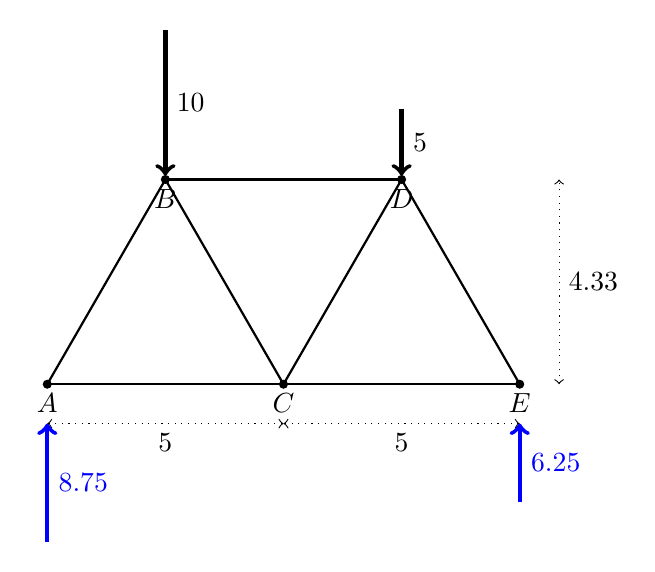
\begin{tikzpicture}
            \coordinate (C) at (0,0);
            \coordinate (E) at (3,0);
            \coordinate (D) at (1.5,2.6);
            \coordinate (B) at (-1.5,2.6);
            \coordinate (A) at (-3,0);

            \draw[fill=black] (C) circle (0.05) node[below]{$C$};
            \draw[fill=black] (E) circle (0.05) node[below]{$E$};
            \draw[fill=black] (D) circle (0.05) node[below]{$D$};
            \draw[fill=black] (B) circle (0.05) node[below]{$B$};
            \draw[fill=black] (A) circle (0.05) node[below]{$A$};

            \draw[thick] (C) -- (E);
            \draw[thick] (E) -- (D);
            \draw[thick] (C) -- (D);
            \draw[thick] (C) -- (B);
            \draw[thick] (C) -- (A);
            \draw[thick] (B) -- (A);
            \draw[thick] (B) -- (D);
            
            \draw[dotted,<->] (-3,-0.5) -- (0,-0.5) node[midway,below] {$5\si{\meter}$};
            \draw[dotted,<->] (3,-0.5) -- (0,-0.5) node[midway,below] {$5\si{\meter}$};
            \draw[dotted,<->] (3.5,0)-- (3.5,2.6) node[midway,right] {$4.33\si{\meter}$};

            \draw[ultra thick,->] (-1.5,4.5) -- (-1.5,2.65) node[midway,right] {$10\si{\kilo\newton}$};
            \draw[ultra thick,->] (1.5,3.5) -- (1.5,2.65) node[midway,right] {$5\si{\kilo\newton}$};
            \draw[color=blue,ultra thick,->] (-3,-2) -- (-3,-0.5) node[midway,right] {$8.75\si{\kilo\newton}$};
            \draw[color=blue,ultra thick,->] (3,-1.5) -- (3,-0.5) node[midway,right] {$6.25\si{\kilo\newton}$};
        \end{tikzpicture}
    \end{center}
    \item We can then solve for the forces in the structure. \textbf{Compression forces} are denoted with a negative number while \textbf{tensile forces} are written with positive numbers.
    \item Beware of \textbf{Euler Buckling}, which is a compression force. The critical load before buckling is:
    \begin{equation}
        P_\text{E}=\frac{\pi^2 EI}{L^2}
        \label{eq:}
    \end{equation}
    
\end{itemize}